%\subsection{Query Transformation}

The main result of this section is the following theorem.
% The main result of this section is an important insight into the mincuts of three vertices captured in the following theorem. This insight will form the foundation for transforming an  edge-containment query in original graph to a more compact graph.


\begin{theorem}
Let $s,r,t\in V$ be any 3 vertices such that $c_{s,r}\ge c_{s,t}$. Let $A\subset V$ define a $(s,t)$-mincut with  $s,r\in A$ and $t\in \overline{A}$. For any subset $E_y$ of edges incident on any vertex $y\in \overline{A}$, there exists a subset $E_A$ of edges from the mincut defined by $A$ such that the following assertion holds.

There is a $(r,s)$-mincut containing $E_y$ if and only if there is a $(r,s)$-mincut containing $E_A$. 
\label{thm:query-transform}
\end{theorem}


\noindent
In order to prove the theorem stated above, we first prove the following lemma.

\begin{lemma}[$3$-vertex Lemma]
Let $s,r,t \in V$ be any three vertices and $c_{r,s} \ge c_{s,t}$. Let $A\subset V$ define an $(s,t)$-mincut as well as
an $(r,t)$-mincut
with $r,s\in A$ and $t\notin A$. Let $B\subset V$ define a $(r,s)$-mincut with $r\in B$. Without loss of generality, assume $t \in {\overline A}\cap {\overline B}$, then the following assertions hold:
\begin{enumerate}
\item
$c(\overline{A}\cap B, A\cap \overline{B})=0$
\item  $A\cap B$ defines a $(r,s)$-mincut.
\item  ${\overline A}\cap {\overline B}$ defines a $(s,t)$-mincut as well as a $(r,t)$-mincut.
\end{enumerate}

For a better illustration refer to Figure \ref{fig:non-S-crossing} ($ii$).
% (Proof in Appendix \ref{appendix:3-vertex-lemma})
\label{lem:3-vertex-lemma}
\end{lemma}

% \section{Proof of Lemma \ref{lem:3-vertex-lemma} (3-vertex lemma)} \label{appendix:3-vertex-lemma}

\begin{proof}
Let $\alpha = c(\bar{A}\cap B, A\cap {B}),
~\beta = c(\bar{A} \cap B, A\cap \bar{B}),~\gamma=c(\bar{A} \cap B, \bar{A}\cap \bar{B})$.
Refer to Figure \ref{fig:non-S-crossing} ($i$) that illustrates these edges and the respective cuts.
\begin{figure}[H]
\centering
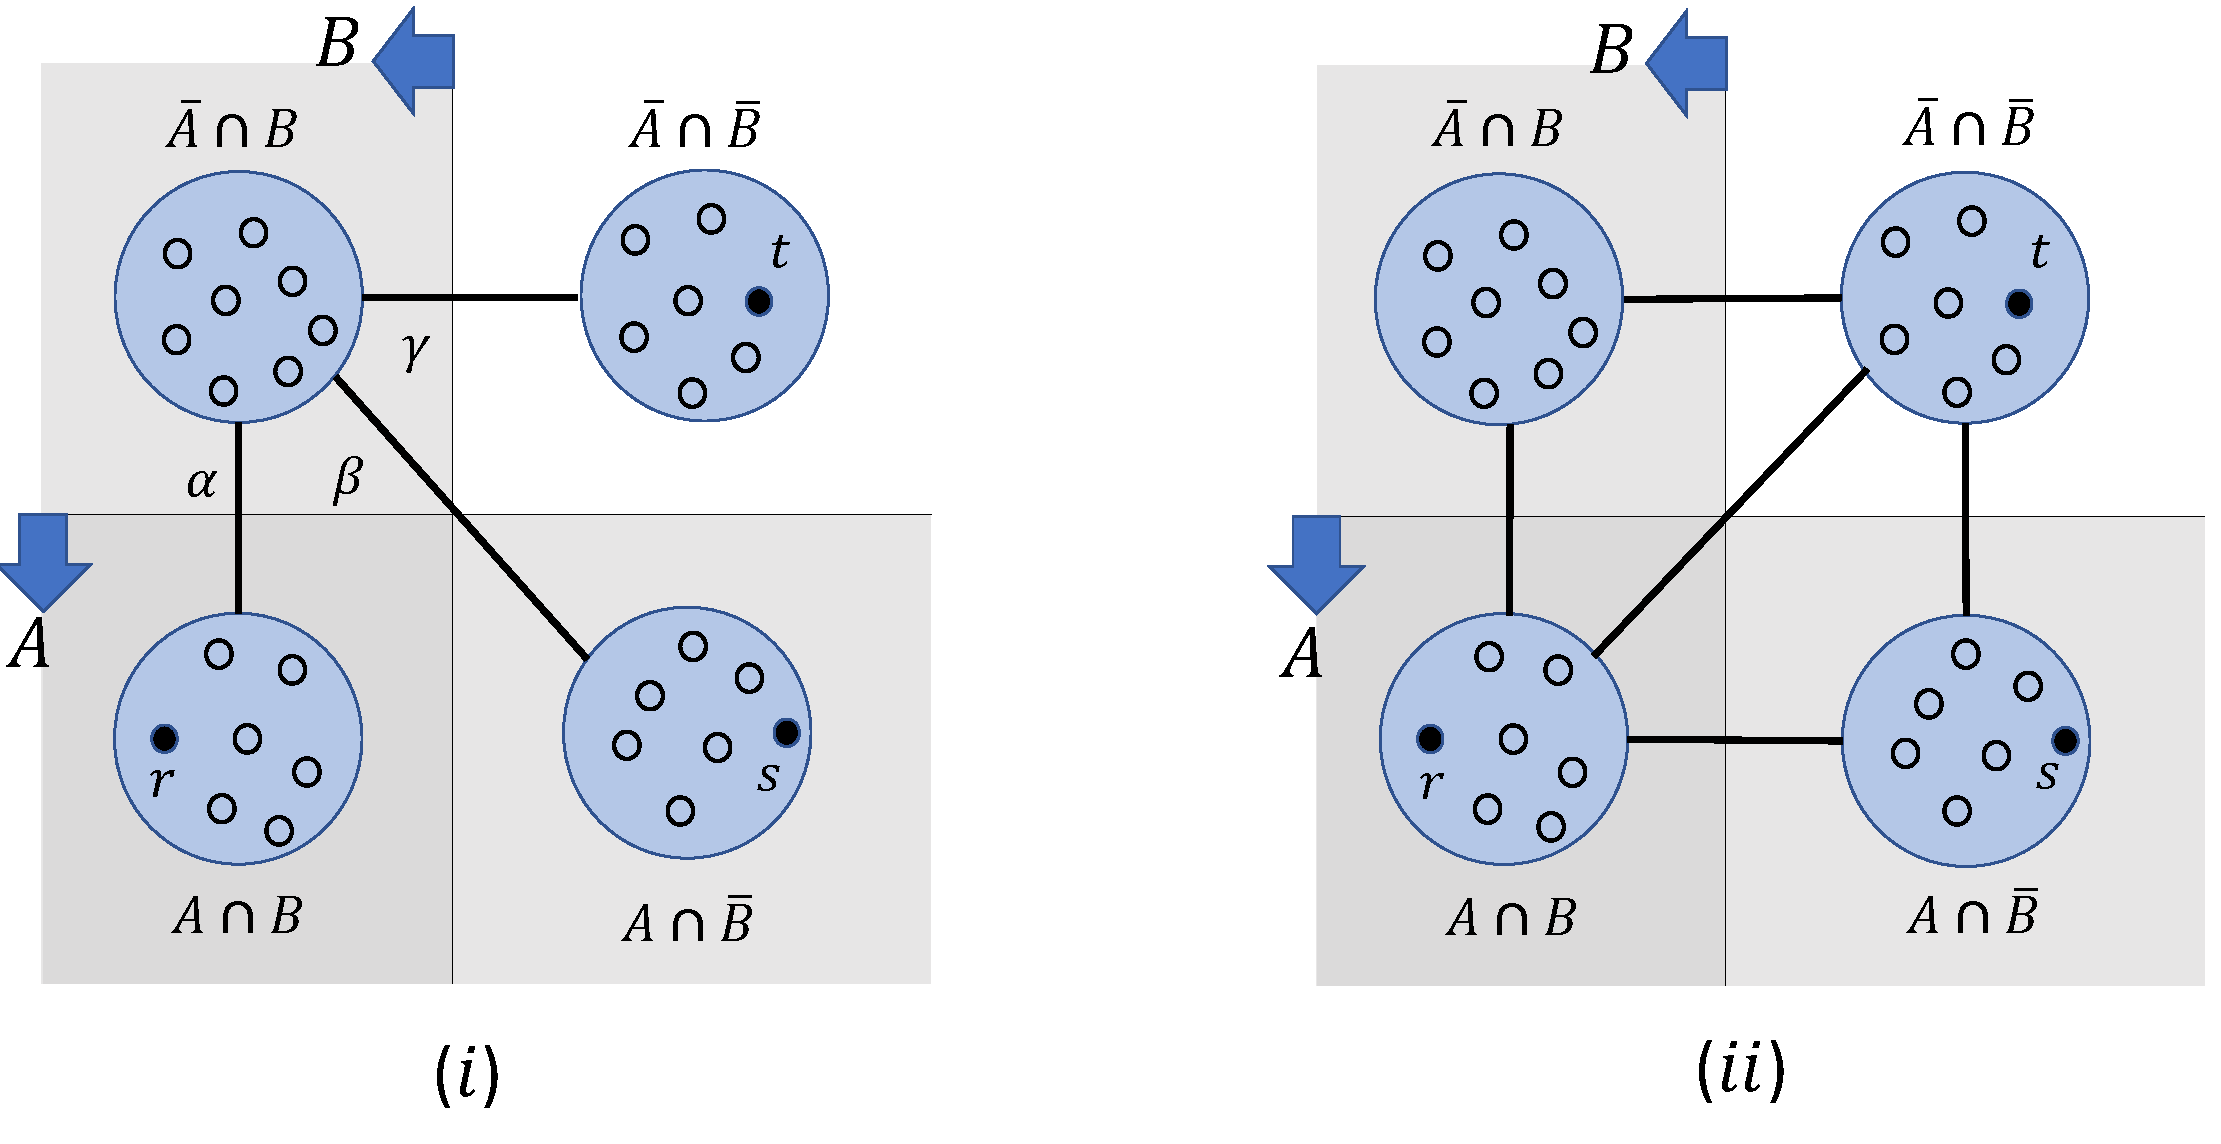
\includegraphics[width=0.75\textwidth]{src/images/S-crossing-and-non-crossing_new.pdf}
    \caption{(i) $\alpha$, $\beta$ and $\gamma$ denote the capacities of edges incident on $\bar{A}\cap B$ from $A\cap B$, $A\cap \bar{B}$, and $\bar{A} \cap \bar{B}$ respectively. (ii) There are no edges along the diagonal between $\bar{A}\cap {B}$ and $A\cap \bar{B}$.}
\label{fig:non-S-crossing}
\end{figure}

Applying Lemma \ref{lem:subset-property-of-min-cut}
on $(s,t)$-mincut with $S=A$ and $S'= \bar{A}\cap B$, we get
\begin{equation}
    \alpha + \beta \le \gamma 
\label{eq:alpha+beta-le-gamma}
\end{equation}
Applying Lemma \ref{lem:subset-property-of-min-cut} on $(r,s)$-mincut with $S=\bar B$ and  $S'= \bar{A} \cap B$, we get $\gamma + \beta \le \alpha$. This inequality combined with Inequality \ref{eq:alpha+beta-le-gamma} implies that $\beta=0$. That is, $c(\bar{A}\cap B, A\cap \bar{B})=0$. This completes the proof of Assertion (1). Refer to Figure \ref{fig:non-S-crossing} (ii) for an illustration. 
It follows from (1) that $\alpha=\gamma$.
That is, $\bar{A} \cap B$ has equal number edges incident from $\bar{A}\cap \bar{B}$ as from $A\cap B$.  This fact can be easily used to infer Assertions (2) and (3) by 
removing $\bar{A}\cap B$ from $B$ and
$\bar{A}$ respectively.
\end{proof}

We shall now establish the proof of Theorem \ref{thm:query-transform}. Suppose $B$ is any $(r,s)$-mincut containing edges $E_y$. Without loss of generality, assume that $r\in B$ and $s,t\notin B$. The following lemma states a crucial property of the cut defined by $A\cup B$ in strip ${\cal D}_{A,t}$, where $\mathbf{s}$ and $\mathbf{t}$ correspond to source $A$ and sink $t$ respectively.
% (Proof in Appendix \ref{appendix:AUB-contains-E_y}).

\begin{lemma}
$A\cup B$ will be a transversal in strip ${\cal D}_{A,t}$, and all edges in $E_y$ are present in this cut.

\label{lem:AUB-contains-E_y}
\end{lemma}
\begin{proof}
It follows from Lemma \ref{lem:3-vertex-lemma}(3) that $A\cup B$ will be a $(s,t)$-mincut. Hence $A\cup B$ will be a transversal in strip ${\cal D}_{A,t}$ that stores all
$(s,t)$-mincuts.
From definition, $y$ belongs to $\bar{A}$. Refer to Figure \ref{fig:non-S-crossing}($ii$).  If $y\in \bar{A}\cap B$, then it follows from Lemma \ref{lem:3-vertex-lemma}(1) that all neighbors of $y$ corresponding to $E_y$ will belong to $\bar{A}\cap \bar{B}$. So $E_y$ belongs to the cut defined by $A\cup B$. The same holds for the case $y\in \bar{A}\cap\bar{B}$ as well since $B\subset A\cup B$.
\end{proof}


It follows from Lemmas \ref{lem:AUB-contains-E_y} and \ref{lem:E_y-edges-same-side} that all edges in $E_y$ must belong to the same side of the inherent partition of the node containing $y$ in strip ${\cal D}_{A,t}$. 
% Otherwise, there is no $(s,r)$-mincut containing $E_y$; so the query
% {\textsc{Edge-Contained}}($s,r,E_y$) can be answered in refutation.
Otherwise, there is no $(r,s)$-mincut which contains set of edges $E_y$. In this case, we can choose $E_A = E(A,{\overline A})$ and Theorem \ref{thm:query-transform} trivially holds.
% {\color{red} Sir, there is some mismatch in $s,t$ and $r,s$ at some places}

Let $x_1,\ldots,x_k$ be the neighbors of $y$ defining $E_y$; that is, $E_y = \{(y,x_i)|
\forall i\in [k]\}$. 
If all edges in $E_y$ lie in side-$\mathbf{s}$,
% If $y$ is on the side of $\mathbf{t}$ in the cut defined by $A\cup B$, 
$R=\bigcup_{i=1}^{k}{\cal R}_s(x_i) \setminus \{\mathbf{s}\}$, that is, the union of the reachability cones of $x_i$'s in the strip ${\cal D}_{A,t}$ towards $\mathbf{s}$ excluding the terminal ${\mathbf{s}}$. If all edges in $E_y$ lie in side-$\mathbf{t}$,
% $y$ is on the side of ${\mathbf{s}}$, 
$R={\cal R}_s(y) \setminus \{\mathbf{s}\}$.
% is defined as the reachability cone of $y$ on the side of $\mathbf{s}$ excluding the terminal $\mathbf{s}$.
We define $E_A$ to be the set of edges which are incident from $R$ to terminal $\mathbf{s}$ as well as those edges in $E_y$ having one endpoint in set $A$. Notice that all edges in set $E_A$
% emanating from $R$ towards terminal $\mathbf{s}$ 
belong to the cut defined by $A$. The following lemma suffices to establish Theorem  \ref{thm:query-transform}.

\begin{lemma}
\label{lem:query-transformation}
\noindent
There is a $(r,s)$-mincut containing edges $E_y$ if and only if there is a $(r,s)$-mincut containing all edges in set $E_A$. 
% emanating from $R$ on the side of $\mathbf{s}$ 
% in strip ${\cal D}_{A,t}$.
\end{lemma}
\begin{proof}
${\cal D}_{A,t}$ stores all $(s,t)$-mincuts that enclose the set $A$ (see Lemma \ref{lem:strip-A}), and thus the mincut defined by $A\cup B$ as well. So all nodes of the strip ${\cal D}_{A,t}$, excluding the terminal node ${\mathbf{s}}$ must remain intact in the cut defined by $B$. Therefore, if we replace the subgraph of $G$ induced by $\overline{A}$ by the strip ${\cal D}_{A,t}$ lying above ${\mathbf{s}}$, the resulting graph, denoted by $G_A$, will preserve all $(r,s)$-mincuts of graph $G$. So in the remaining part of this proof, %henceforth we may focus 
we focus on $G_A$ instead of $G$. 
Let us consider the case when $E_y$ is on side-$\mathbf{s}$.
%all $x_i's$ are on the side of $\mathbf s$ from $y$. 
The proof for the other case will follow likewise.

Let $B$ be a $(r,s)$-mincut containing edges $\{(y,x_1),\ldots,(y,x_k)\}$.
%Without loss of generality, assume that $t\notin B$.
Refer to Figure \ref{fig:B-crosses-A}($ii$) that demonstrates $A$ and $B$ in the graph $G_A$.
Observe that $y$ does not belong to $A$, so $\{x_1,\ldots,x_k\}\subset A\cup B$.
Since $A\cup B$ is a transversal in ${\cal D}_{A,t}$, so $R\subset A\cup B$. It follows from the construction that $R$ lies totally outside $A$, therefore, $R$ must lie fully inside $\overline{A}\cap B$. Using this fact and Lemma \ref{lem:3-vertex-lemma} (1), all edges emanating from $R$ on the side of $\mathbf{s}$
are incident only on $A\cap B$. But $A\cap B$ defines a $(r,s)$-mincut as follows from Lemma \ref{lem:3-vertex-lemma} (2). 
%This cut is obtained by removing $\overline{A}\cap B$ from $B$. So it follows that $R$ lies outside $A\cap B$ and $R$ contributes all outgoing edges to the cut defined by $A\cap B$. 
Furthermore, the cut defined by $A\cap B$ also contains all edges in $E_y$ that have one endpoint in $A$.
Thus, $A\cap B$ is the desired $(r,s)$-cut since it contains all edges in $E_A$.
\begin{figure}[h]
    \centering
    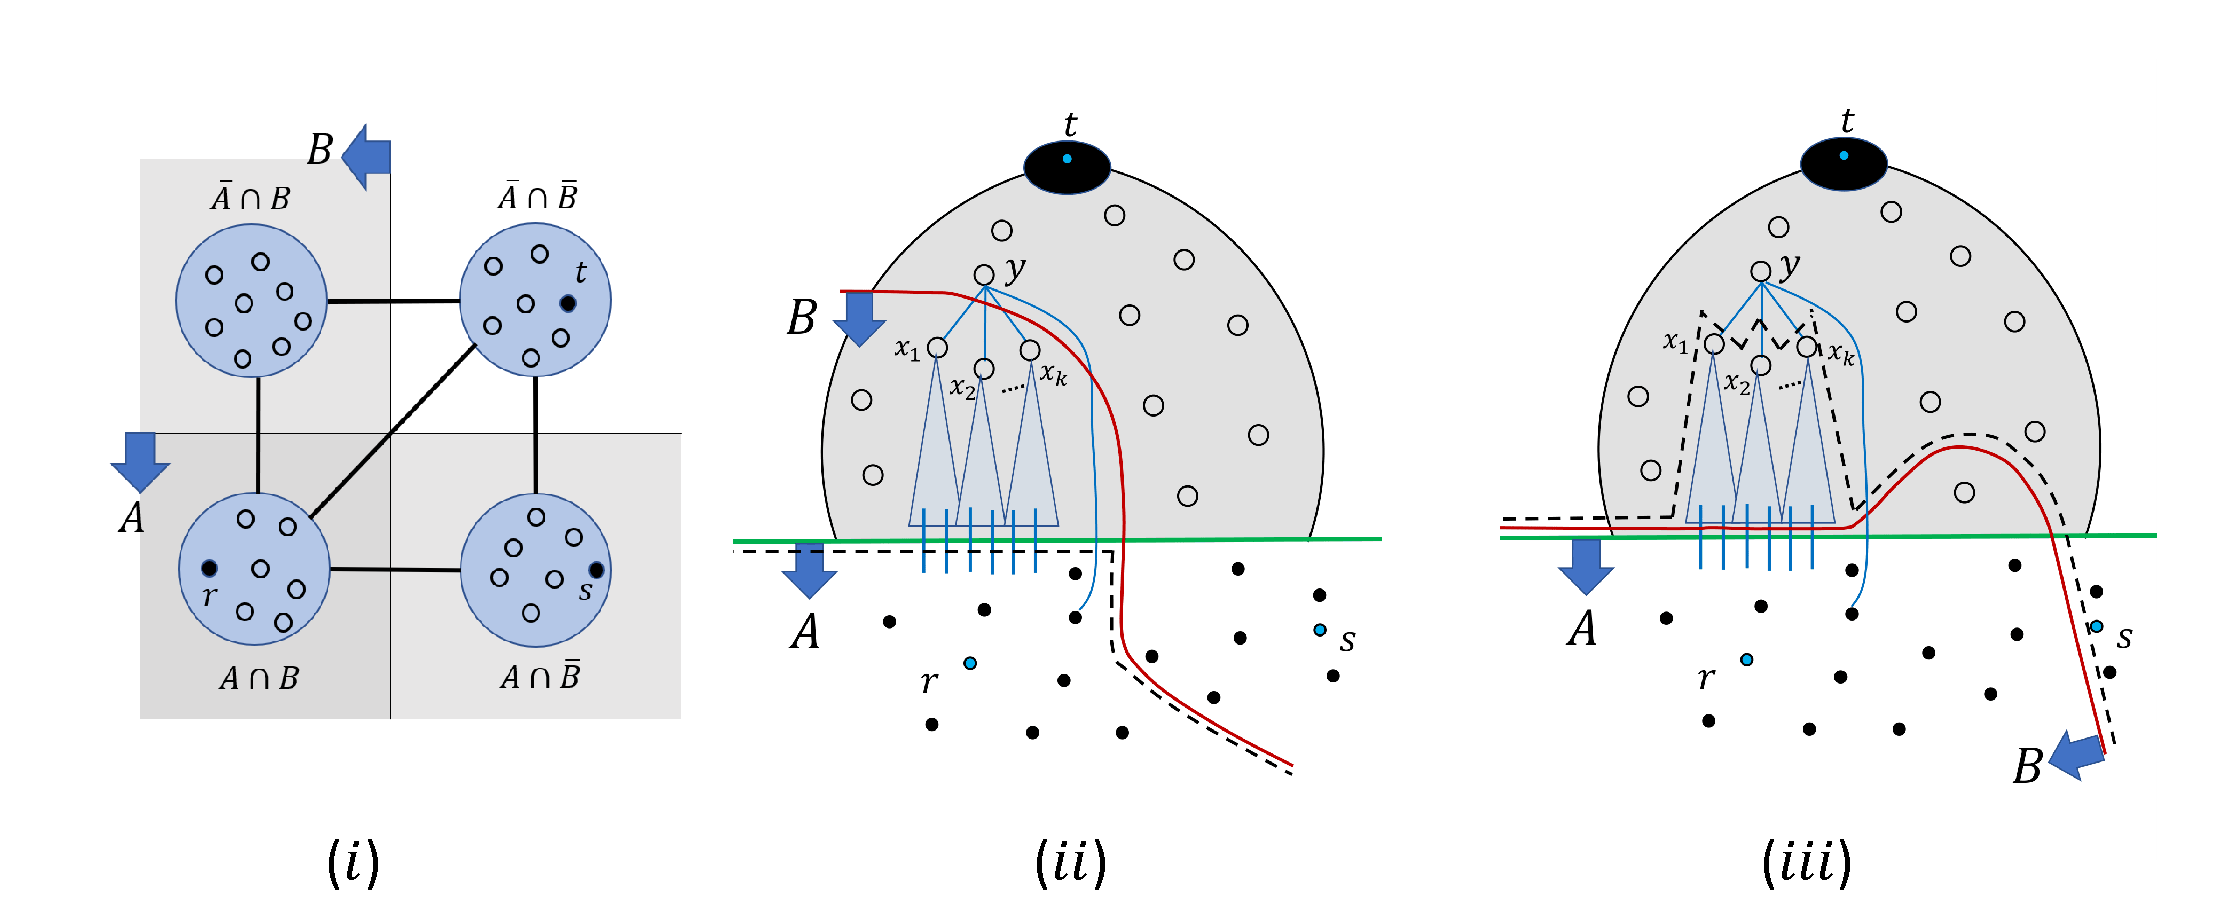
\includegraphics[width=\textwidth]{src/images/compressed-image-i-ii.pdf}{}
    \caption{($i$) There are no edges along the diagonal between $\overline{A}\cap {B}$ and $A\cap \overline{B}$.~($ii$) $B$ cuts edges $\{(y,x_1),\ldots,(y,x_k)\}$.~$(iii)$ $B$ cuts all outgoing edges of $R$.}
    \label{fig:B-crosses-A}
\end{figure}

Let $B$ be a $(r,s)$-mincut that cuts all edges in set $E_A$.
% emanating from $R$ on the side of $\mathbf{s}$. 
Refer to Figure \ref{fig:B-crosses-A}($iii$). By construction $R$ lies outside $A$ 
% and the cut defined by $A$ cuts all edges in $E_A$.
and all edges in $E_y$ with one endpoint in $A$ are contained in the cut defined by $A\cup B$.
% emanating from $R$ on the side of $\mathbf{s}$.
 Therefore, the cut defined by $A\cup B$ cuts all edges in $E_A$.
%  emanating from $R$ on the side of $\mathbf{s}$. 
Since $A\cup B$ is a transversal in ${\cal D}_{A,t}$, it follows that $(A\cup B) \cap R = \emptyset$; otherwise it would imply a coherent path in strip ${\cal D}_{A,t}$ that intersects $A\cup B$ twice -- a contradiction. So $B \cap R = \emptyset$ too. That is, $R$ lies entirely on the side of $t$ in the cut defined by $B$. Treating $R$ as a single vertex, observe that its incoming edges are the same in number as its outgoing edges in ${\cal D}_{A,t}$. It is given that $R$ currently contributes all its outgoing edges to the cut defined by $B$. So it follows that $B\cup R$, which also defines a $(r,s)$-cut, has the same capacity as $B$, but $R$ now contributes all incoming edges to this cut. 
 %Now observe that $r$ belongs to $B\cup R$ since $r$ is in $B$ by construction. $s$ does not belong to $B \cup R$ since, by construction, $s$ is neither in $R$ nor in $B$. 
 So $B\cup R$ is the desired $(r,s)$-mincut containing edges $(y,x_1),\ldots,(y,x_k)$.
 %It follows from above that all incoming edges of $R$ contribute to this cut. So the cut defined by $B\cup R$ cuts all edges $(y,x_1),…,(y,x_k)$. So $B\cup R$ is the desired $(r,s)$-cut.
\end{proof}

% In fact, if we have a $(r,s)$-mincut that cuts all edges in $E_A$, we can construct a $(r,s)$-mincut that cuts all edges in $E_y$. We have already given the construction in Proof of Lemma \ref{lem:query-transformation}. We state this result in the following corollary.

% It follows from the construction in Proof of Lemma \ref{lem:query-transformation}, that given a $(r,s)$-mincut that contains all edges in $E_A$ we can construct another $(r,s)$-mincut that contains all edges in $E_y$.
The following corollary follows from the construction in Proof of Lemma \ref{lem:query-transformation}.

\begin{corollary}
\label{cor:query-transformation}
Given a $(r,s)$-mincut that contains all edges in $E_A$ another $(r,s)$-mincut can be constructed that contains all edges in $E_y$.
% Suppose $B$ is a $(r,s)$-mincut such that $s,t\in {\overline B}$ and it contains all edges in set $E_A$. The set of vertices $B\cup R$ defines a $(r,s)$-mincut that cuts all edges in $E_y$.
\end{corollary}

\section{Insights into Nearest Mincuts}
\label{sec:insights-nearest-mincuts}

Let $s,r,t \in V$ be any $3$ vertices such that $c_{s,r} \geq c_{s,t}$. Let $A\subset V$ define a $(s,t)$-mincut with $s,r \in A$ and $t\in {\overline A}$. Suppose $y \in {\overline A}$ be another vertex. Suppose $G_A$ is the graph obtained by compressing the set ${\overline A}$ to a single vertex. To keep the ideas simple, we shall denote this compressed vertex by ${\overline A}$. Using the notations from \ref{sec:prelimiaries}, sets $s_r^N$ and $r_s^N$ define the nearest $(s,r)$-mincut from $s$ to $r$ and $r$ to $s$ respectively in graph $G$. We state the following lemma. The proof follows from the definition of nearest mincuts.

\begin{lemma}
\label{lem:y-in-nearest-(r,s)-G_A}
If $y$ lies in nearest $s$ to $r$ mincut in $G$, then ${\overline A}$ lies in nearest $s$ to $r$ mincut in $G_A$.
\end{lemma}
\begin{proof}
We know that each $(s,r)$-mincut defined by $(B, {\overline B})$ in $G_A$ is also a $(s,r)$-mincut in $G$. Suppose $\overline{A} \not \in B$ and $s \in B$ where $(B,{\overline B})$ define nearest $s$ to $r$ mincut. Thus, $y \not \in B$. Therefore, $y$ does not lies in nearest $s$ to $r$ mincut in $G$. 
\end{proof}
% Another important observation can be derived from Lemma \ref{lem:3-vertex-lemma}. We can state the following lemma.

% \begin{lemma}
% ${\overline A}$ lies in nearest $r$ to $s$ mincut in $G_A$ if and only if $t \in r_s^N$.
% \end{lemma}

Suppose $\mathbf s$ and $\mathbf t$ correspond to source $A$ and sink $t$ respectively of strip ${\cal D}_{A,t}$. Suppose $R={\cal R}_s(y)\setminus\{\mathbf{s}\}$ denote the set of vertices that form the reachability cone of $y$ towards source $\mathbf s$ in this strip (excluding $\mathbf s$). We define $E_A$ to be the set of edges which are incident from $R$ to terminal $\mathbf s$. We state the following lemma which concisely captures the condition for $y$ to lie in nearest $s$ to $r$ mincut.



\begin{lemma}

\label{lem:y-in-nearest-r-s-mincut}
$y$ lies in the nearest $s$ to $r$ mincut in $G$ if and only if the following conditions hold:

\begin{enumerate}
    \item ${\overline A}$ lies in nearest $s$ to $r$ mincut in $G_A$.
    \item There is no $(s,r)$-mincut that contains all edges in $E_A$.
\end{enumerate}
\end{lemma}
\begin{proof}
The first proposition follows from Lemma \ref{lem:y-in-nearest-(r,s)-G_A}. Thus, in the following analysis, we shall assume that ${\overline A}$ lies in nearest $s$ to $r$ mincut in $G_A$. Suppose $({\overline B},B)$ defines the nearest $s$ to $r$ mincut in $G$. It follows from \ref{lem:3-vertex-lemma} that $t\in {\overline B}$, otherwise $A\cap {\overline B}$ will define a $s$ to $r$ mincut which does not contain ${\overline A}$. 

Suppose $y$ does not lies in nearest $s$ to $r$ mincut i.e. $y \in {\overline A} \cap B$. In this case $R \subset {\overline A} \cap B$. Thus, $A\cap {\overline B}$ defines a $(s,r)$-mincut that contains all edges in $E_A$. Thus, if $E_A$ does not lies in some $(s,r)$-mincut, $y$ lies in nearest $s$ to $r$ mincut.

Now, consider the other direction of this proof. Suppose $y$ lies in nearest $s$ to $r$ mincut. Suppose $y \in \mathbf{t}$, in this case trivially there is no $(s,r)$-mincut that contains all edges in $E_A$ (note that $R = {\overline A}$ in this case). Thus, assume $y$ is a non-terminal in strip ${\cal D}_{A,t}$. Suppose there exists a $(s,r)$-mincut defined by set of vertices $B$ such that it cuts all edges in $E_A$ and $s,t \in {\overline B}$. By construction $R$ lies outside $A$ and all edges in $E_A$ are contained in the cut defined by $A\cup {B}$. Since $A\cup {B}$ is a transversal in ${\cal D}_{A,t}$, it follows that $(A\cup {B}) \cap R = \varnothing$; otherwise it would imply a coherent path in strip ${\cal D}_{A,t}$ that intersects $A \cup {B}$ twice -- a contradiction. So $B\cap R = \varnothing$ too. That is, $R$ lies entirely in the side of $s$ in the cut defined by $B$. Treating $R$ as a single vertex, observe that its incoming edges are the same in number as its outgoing edges in ${\cal D}_{A,t}$. Since $R$ contributes all its outgoing edges in cut defined by $B$, it follows that $B\cup R$ also defines a $(s,r)$-mincut. Clearly, $y \not\in {\overline {B \cup R}}$. Thus, $(\overline{B\cup R}, B\cup R)$ defines a $(s,r)$-mincut in which $y$ is not on the side of $s$ -- a contradiction. Therefore, if $y$ lies in nearest $s$ to $r$ mincut, no $(s,r)$-mincut contains all edges in $E_A$.

\end{proof}

Now, the following lemma can be seen as a corollary of Lemma \ref{lem:query-transformation} and \ref{lem:y-in-nearest-r-s-mincut}.

\begin{corollary}

\label{cor:y-lies-in-nearest-r-s-mincut}

$y$ lies in the nearest $s$ to $r$ mincut in $G$ if and only if the following conditions hold:

\begin{enumerate}
    \item ${\overline A}$ lies in nearest $s$ to $r$ mincut in $G_A$.
    \item There is no $(s,r)$-mincut that contains all edges in side-$\mathbf{s}$ of $y$.
\end{enumerate}
\end{corollary}